\section{ガイド磁場コイル}
ガイド磁場コイルには二つの役割を持っている:
\begin{enumerate}
\item 実験装置全体に渡って中性子の量子化軸を定める
\item 垂直方向に地磁気を無視できる程の大きさの磁場を一様に印加する
\end{enumerate}

特に二つ目の役割は重要であり、磁場の大きさが地磁気に比べて十分大きくないと地磁気によるスピンの反転が起きてしまうことになる。
図\ref{device_fig_guide}はガイド磁場コイルに1Aの電流を流したときの磁場分布シミュレーション結果である。このシミュレーションから得られた$y,z$方向それぞれ$\pm0.04$mの範囲における磁場の不均一性は$y$方向が2.5\% $z$方向が1.6\% 程度に抑えられており、この磁場の一様性は中性子が通過する場所によって干渉条件が大きくずれないことを保証する。
実験ではガイド磁場コイルに5.5Aの電流を流し、ビーム軸上で磁場の強さは約12.8Gとなった。
なお電流を5.5A流すとガイド磁場コイルの温度が60$^\circ$C以上になる部分もあったため、3台の扇風機で空冷しながら実験を行った。
\begin{figure}[H]
\begin{center}
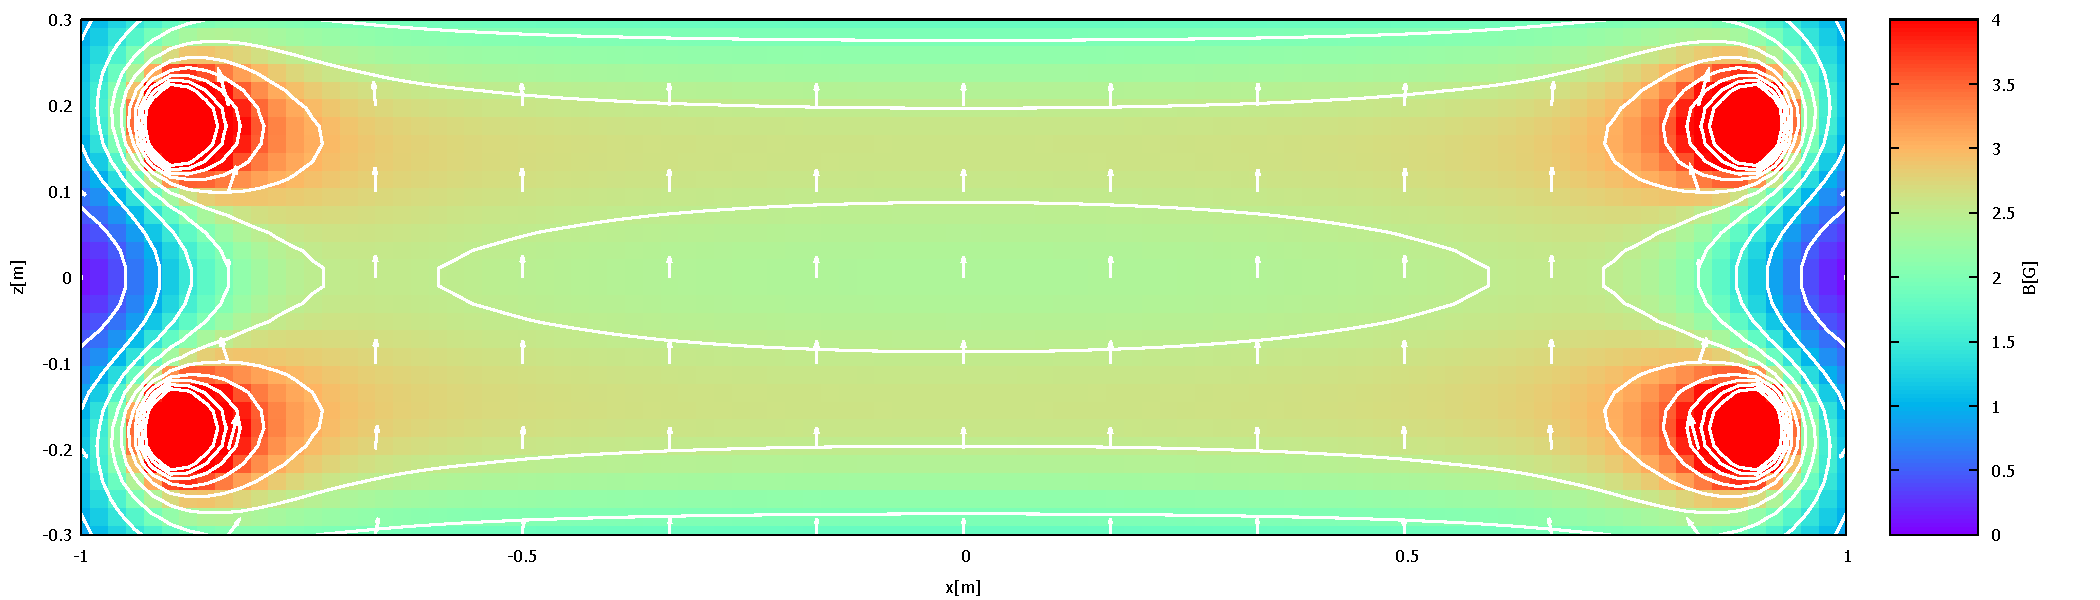
\includegraphics[width=12cm]{device/coil4_image1.pdf}
\subcaption{横から}
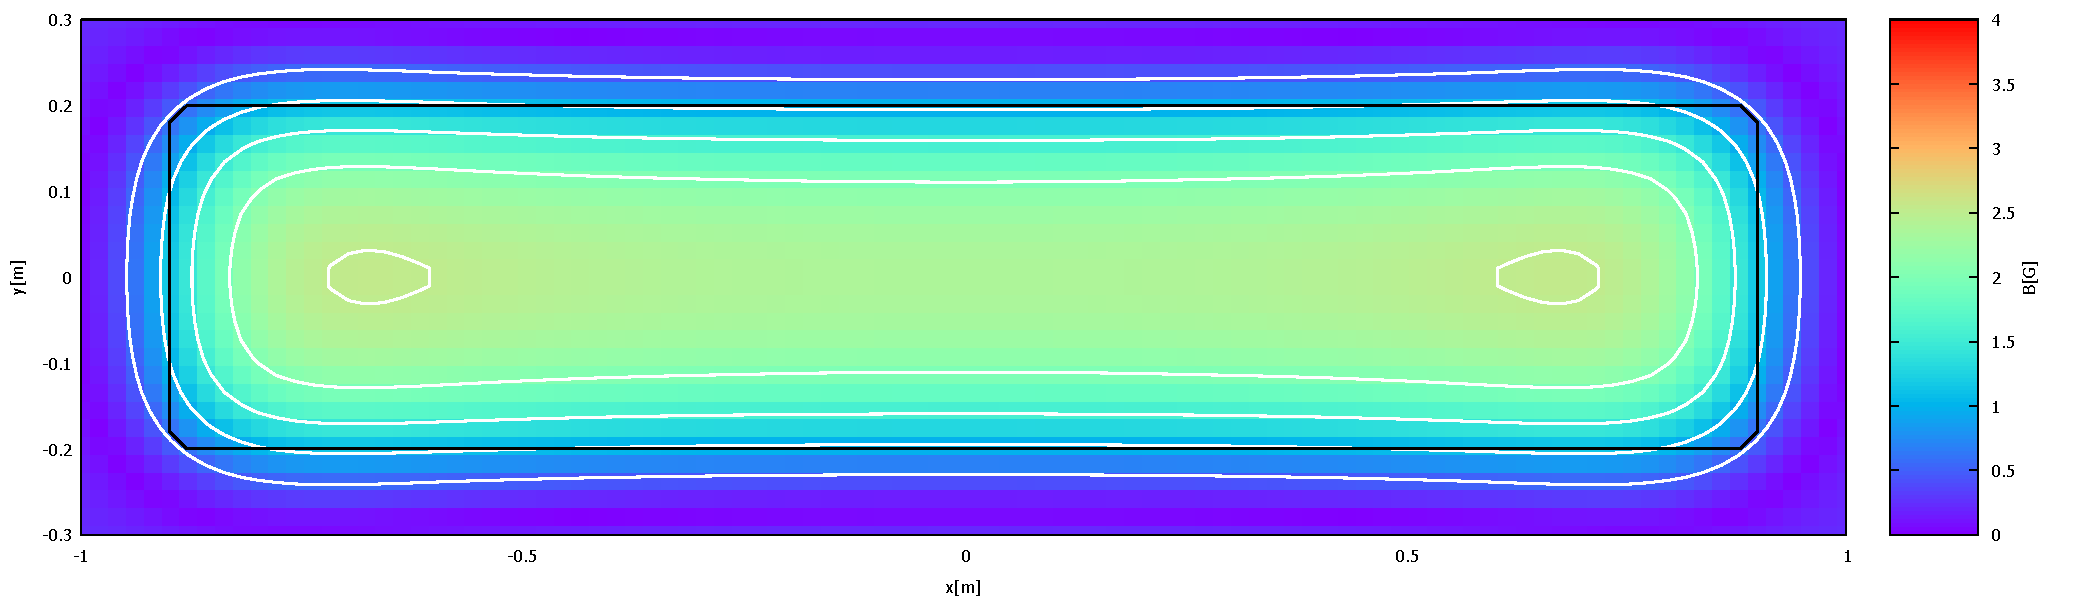
\includegraphics[width=12cm]{device/coil4_image2.pdf}
\subcaption{上から}
\end{center}
\caption{ガイド磁場コイルの磁場分布シミュレーション}\label{device_fig_guide}
\end{figure}
\begin{figure}[H]
\centering
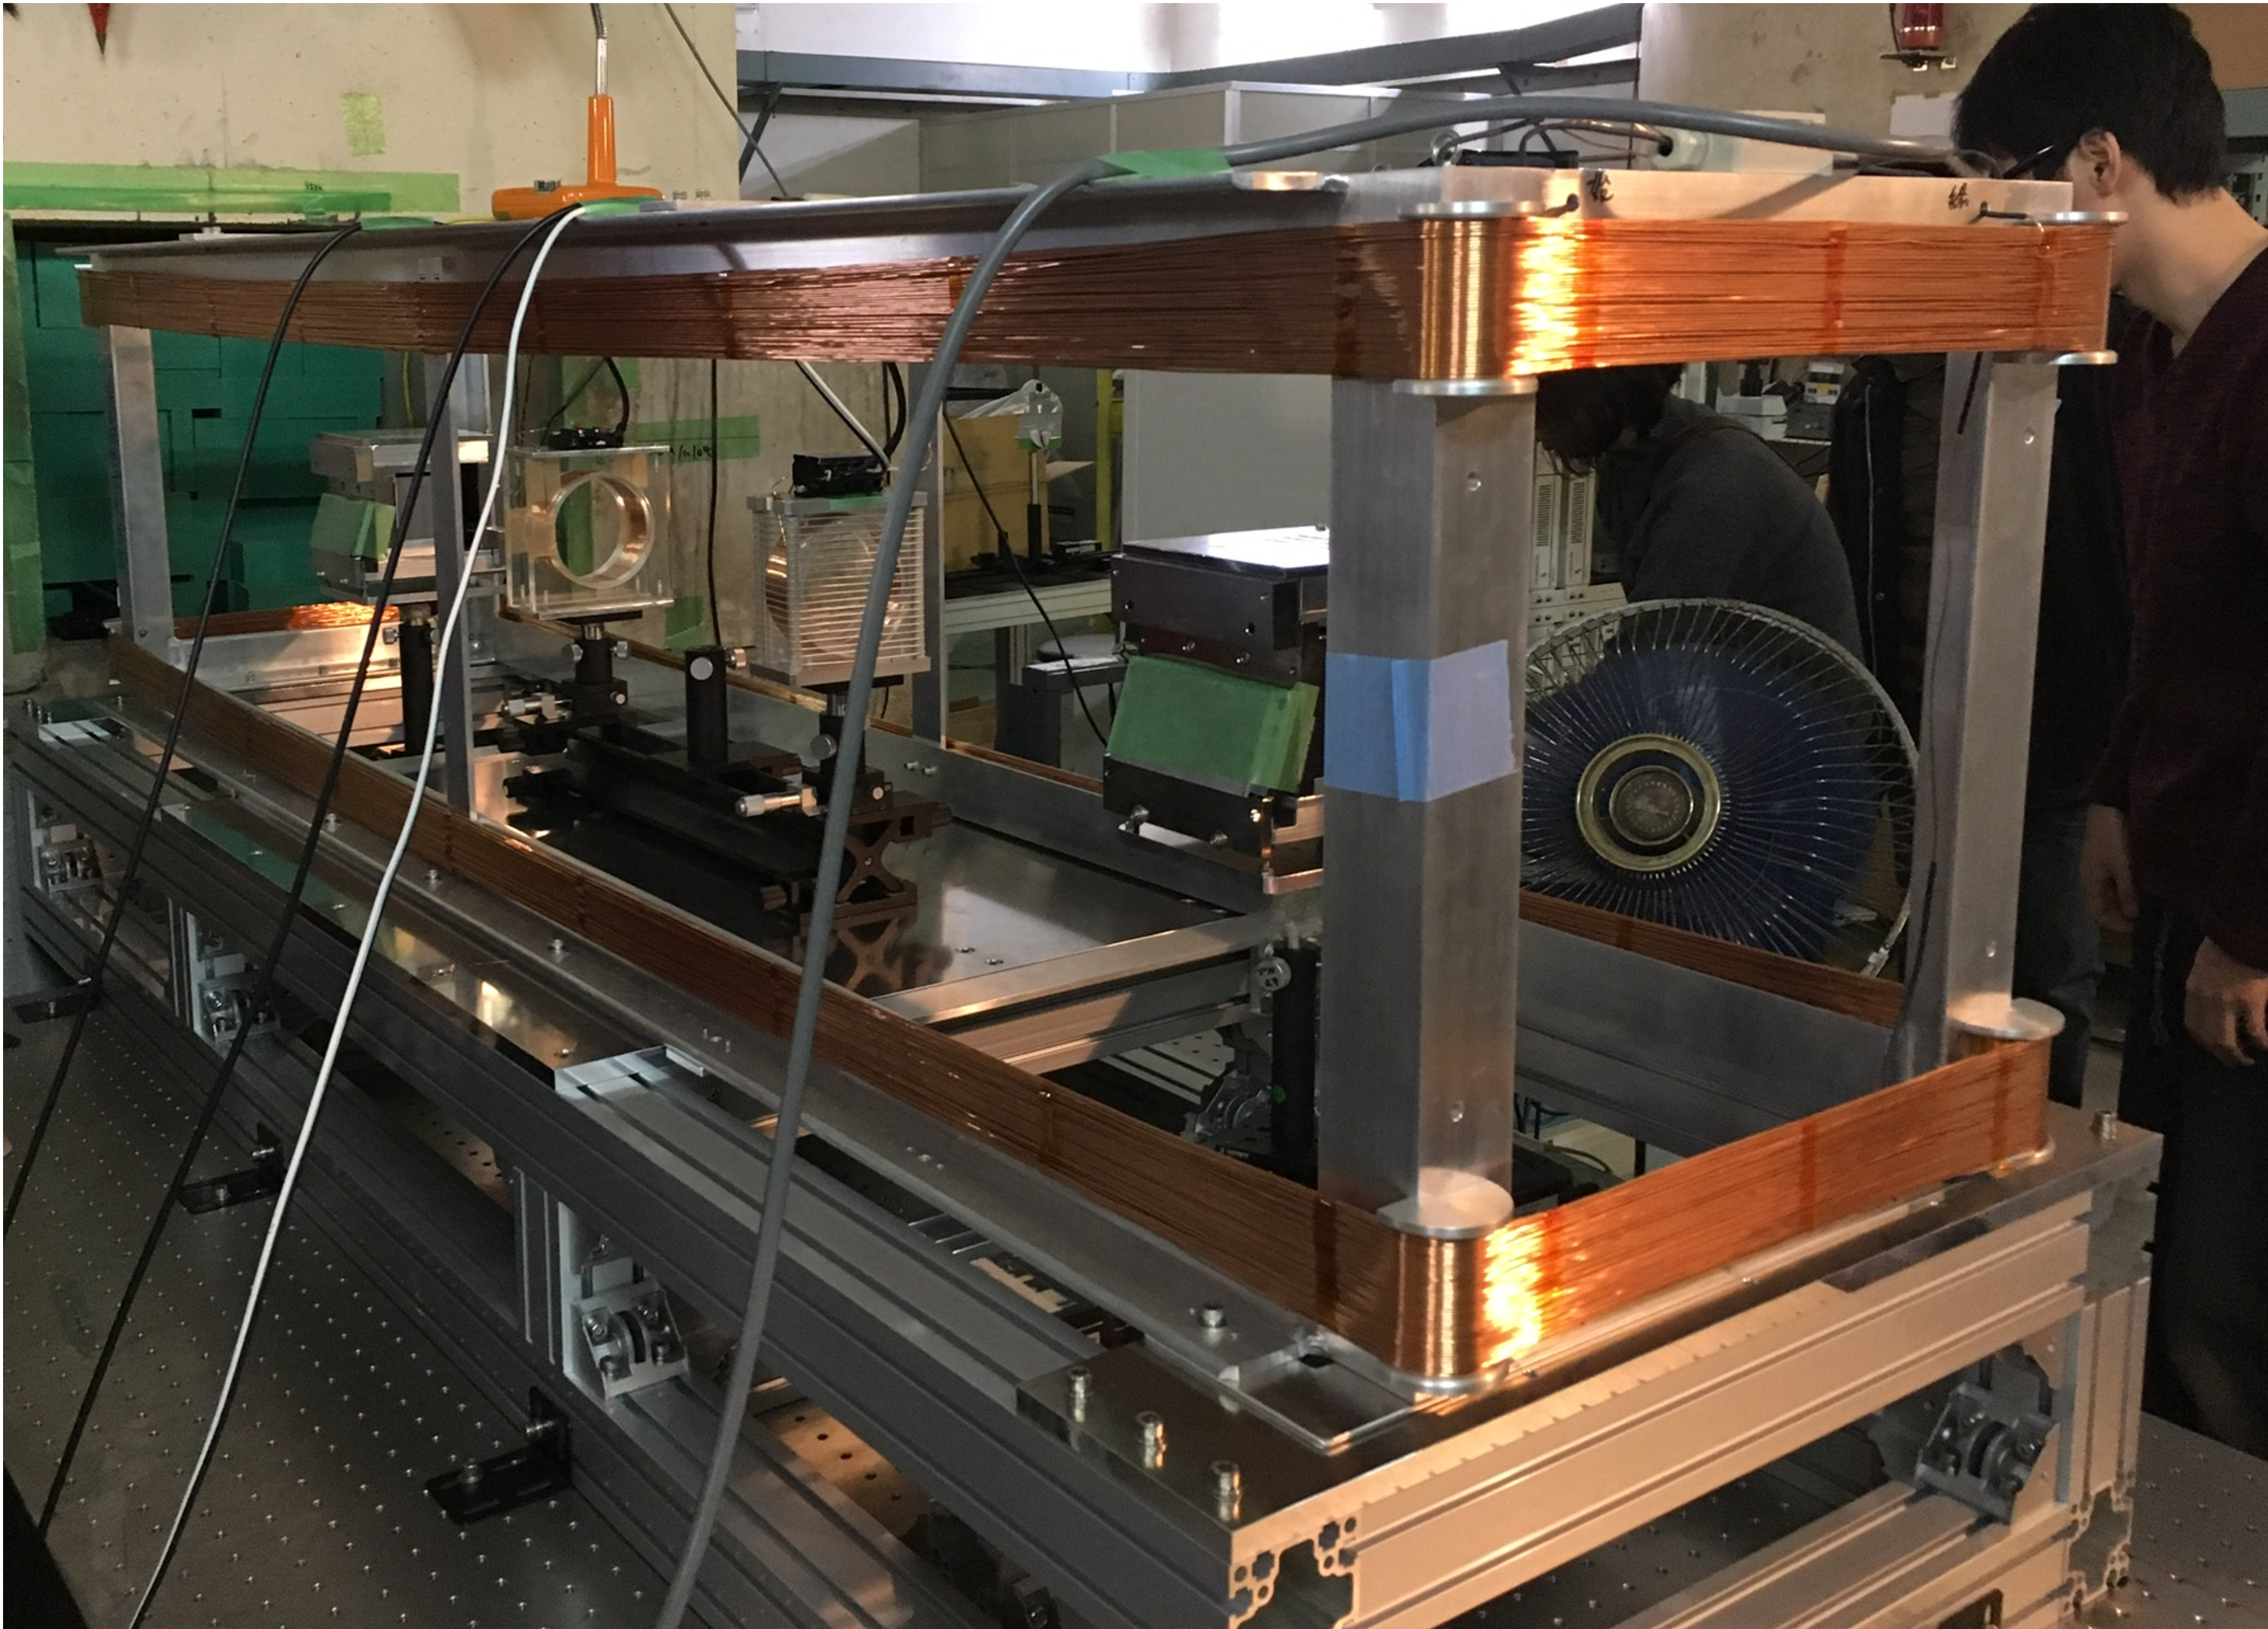
\includegraphics[width=8cm,height=5cm]{device/coilphoto.pdf}\caption{ガイド磁場コイル}
\end{figure}

\begin{comment}
\section{磁気スーパーミラー}
磁気スーパーミラーは入射した中性子のうちスピン上向きのみを選択的に取り出す役割を持つ。膜厚を少しずつ変えた多層膜により全反射とBragg反射の両方を利用して幅広いエネルギーの中性子を反射することができる。反射の詳しい原理は\ref{mirror_sec}章で述べる。
\begin{figure}[H]
\centering
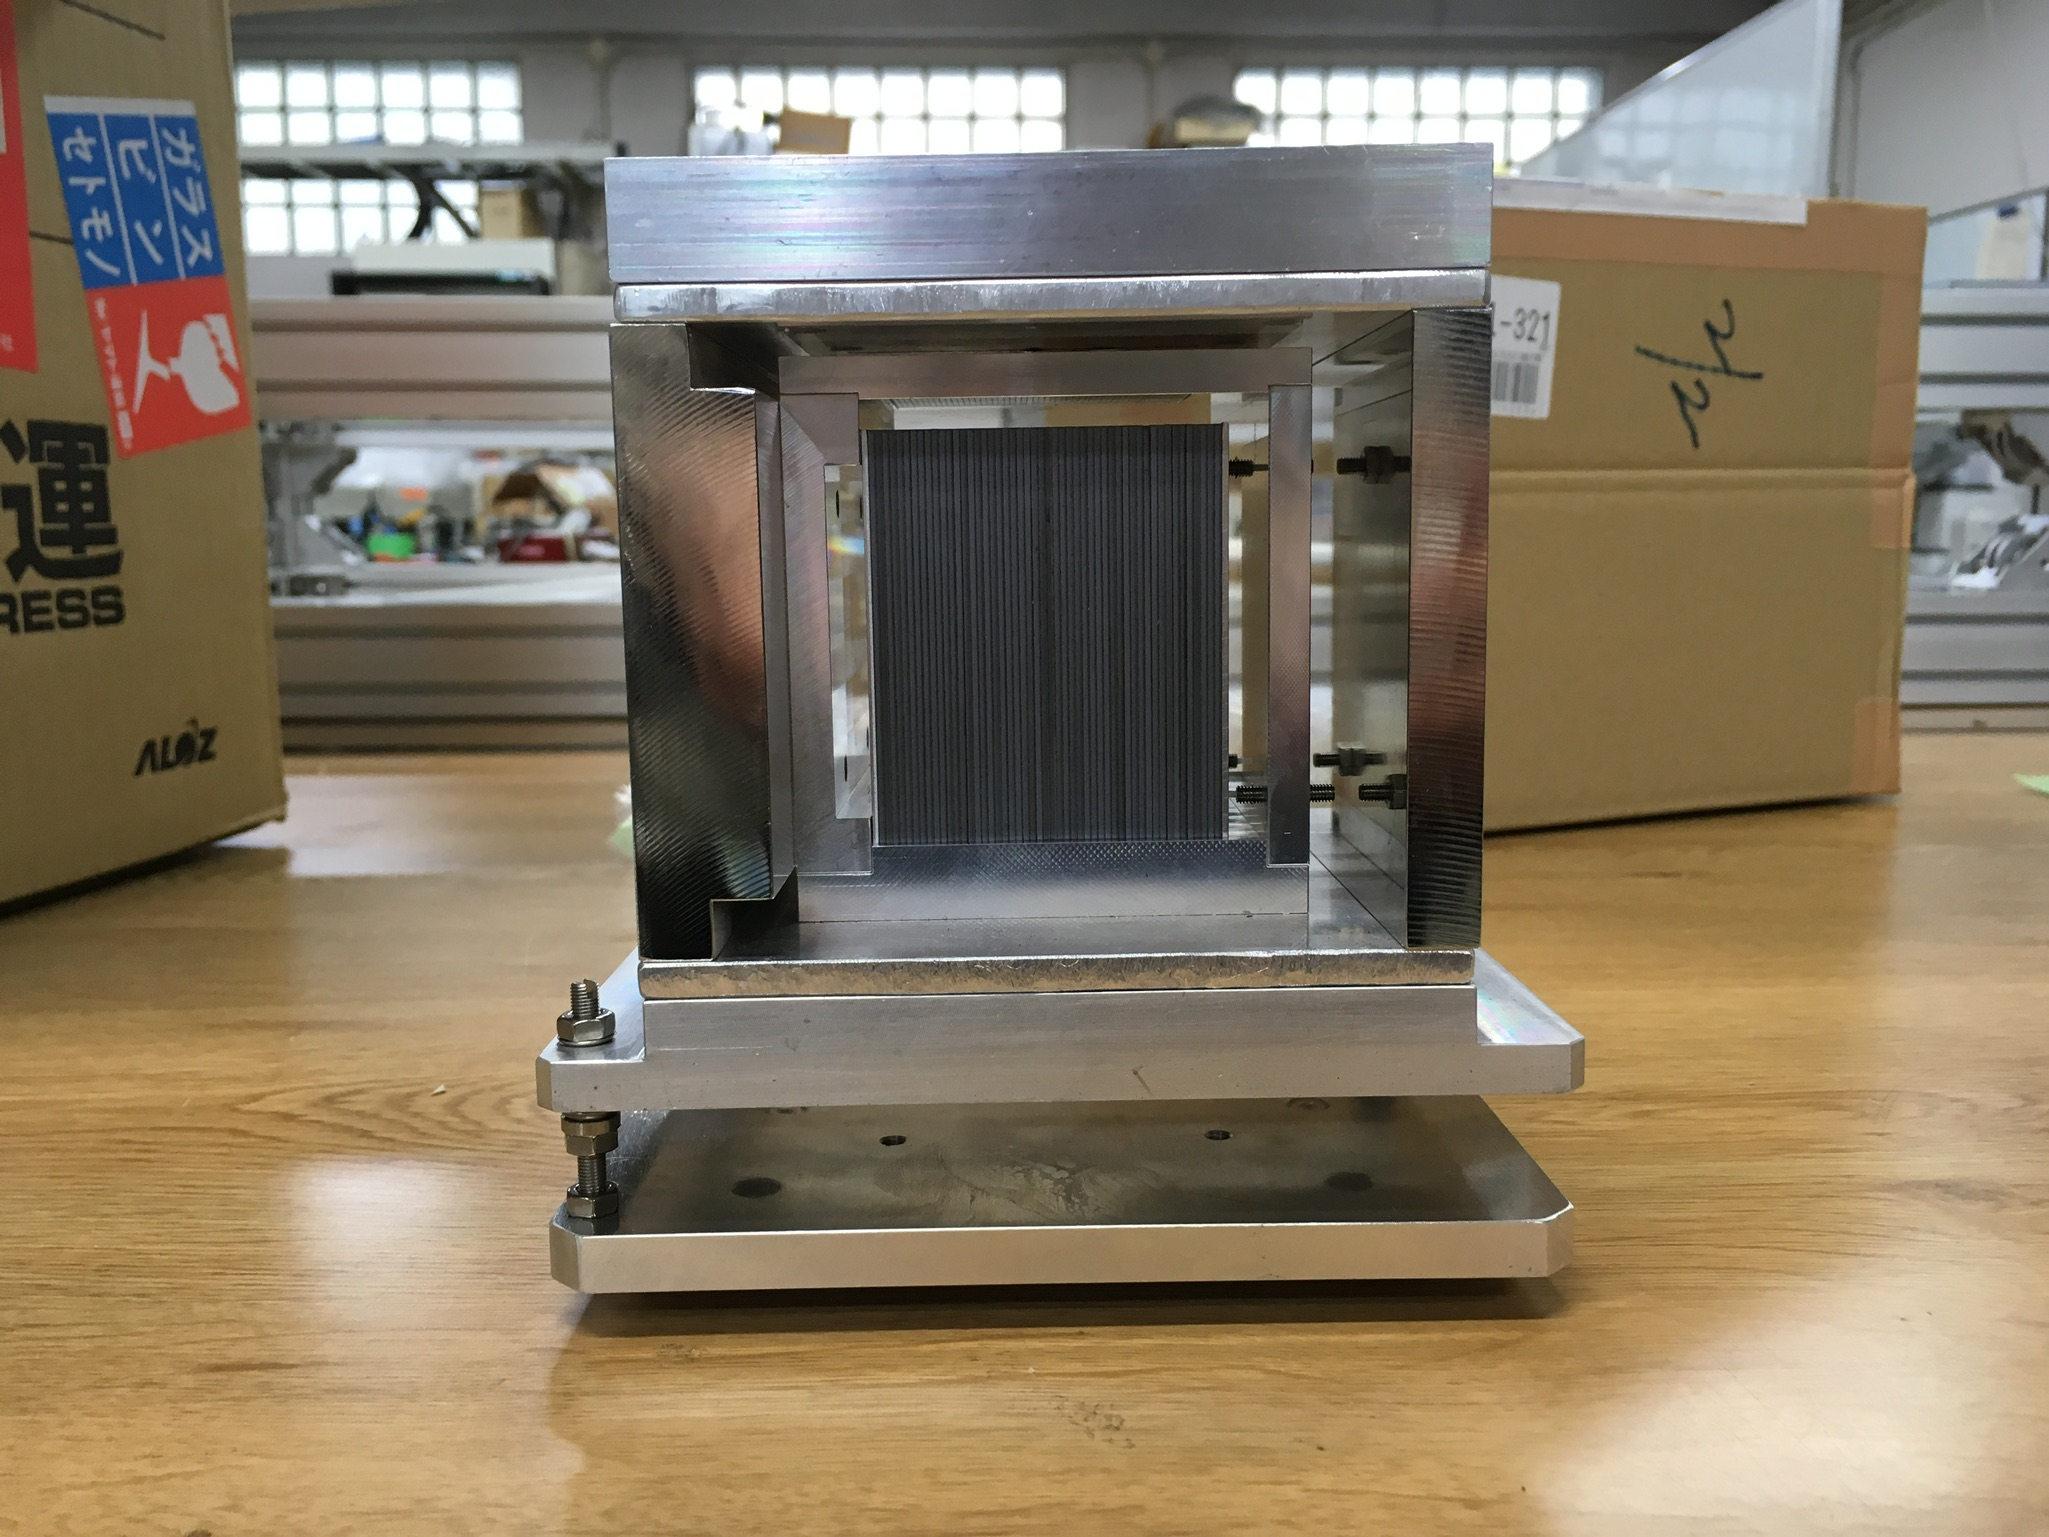
\includegraphics[width=8cm]{device/mirrorphoto.jpg}\caption{磁気スーパーミラー}
\end{figure}
\end{comment}

\section{スピンフリッパ―}
スピンフリッパ―は入射中性子をスピン上向きと下向きの状態の重ね合わせにする役割を持っている。
装置としての構造は極めて単純で普通のソレノイドコイルである。コイルに高周波電流を流すことによって高周波磁場を作り出しスピンをフリップさせている。
\begin{figure}[H]
\centering
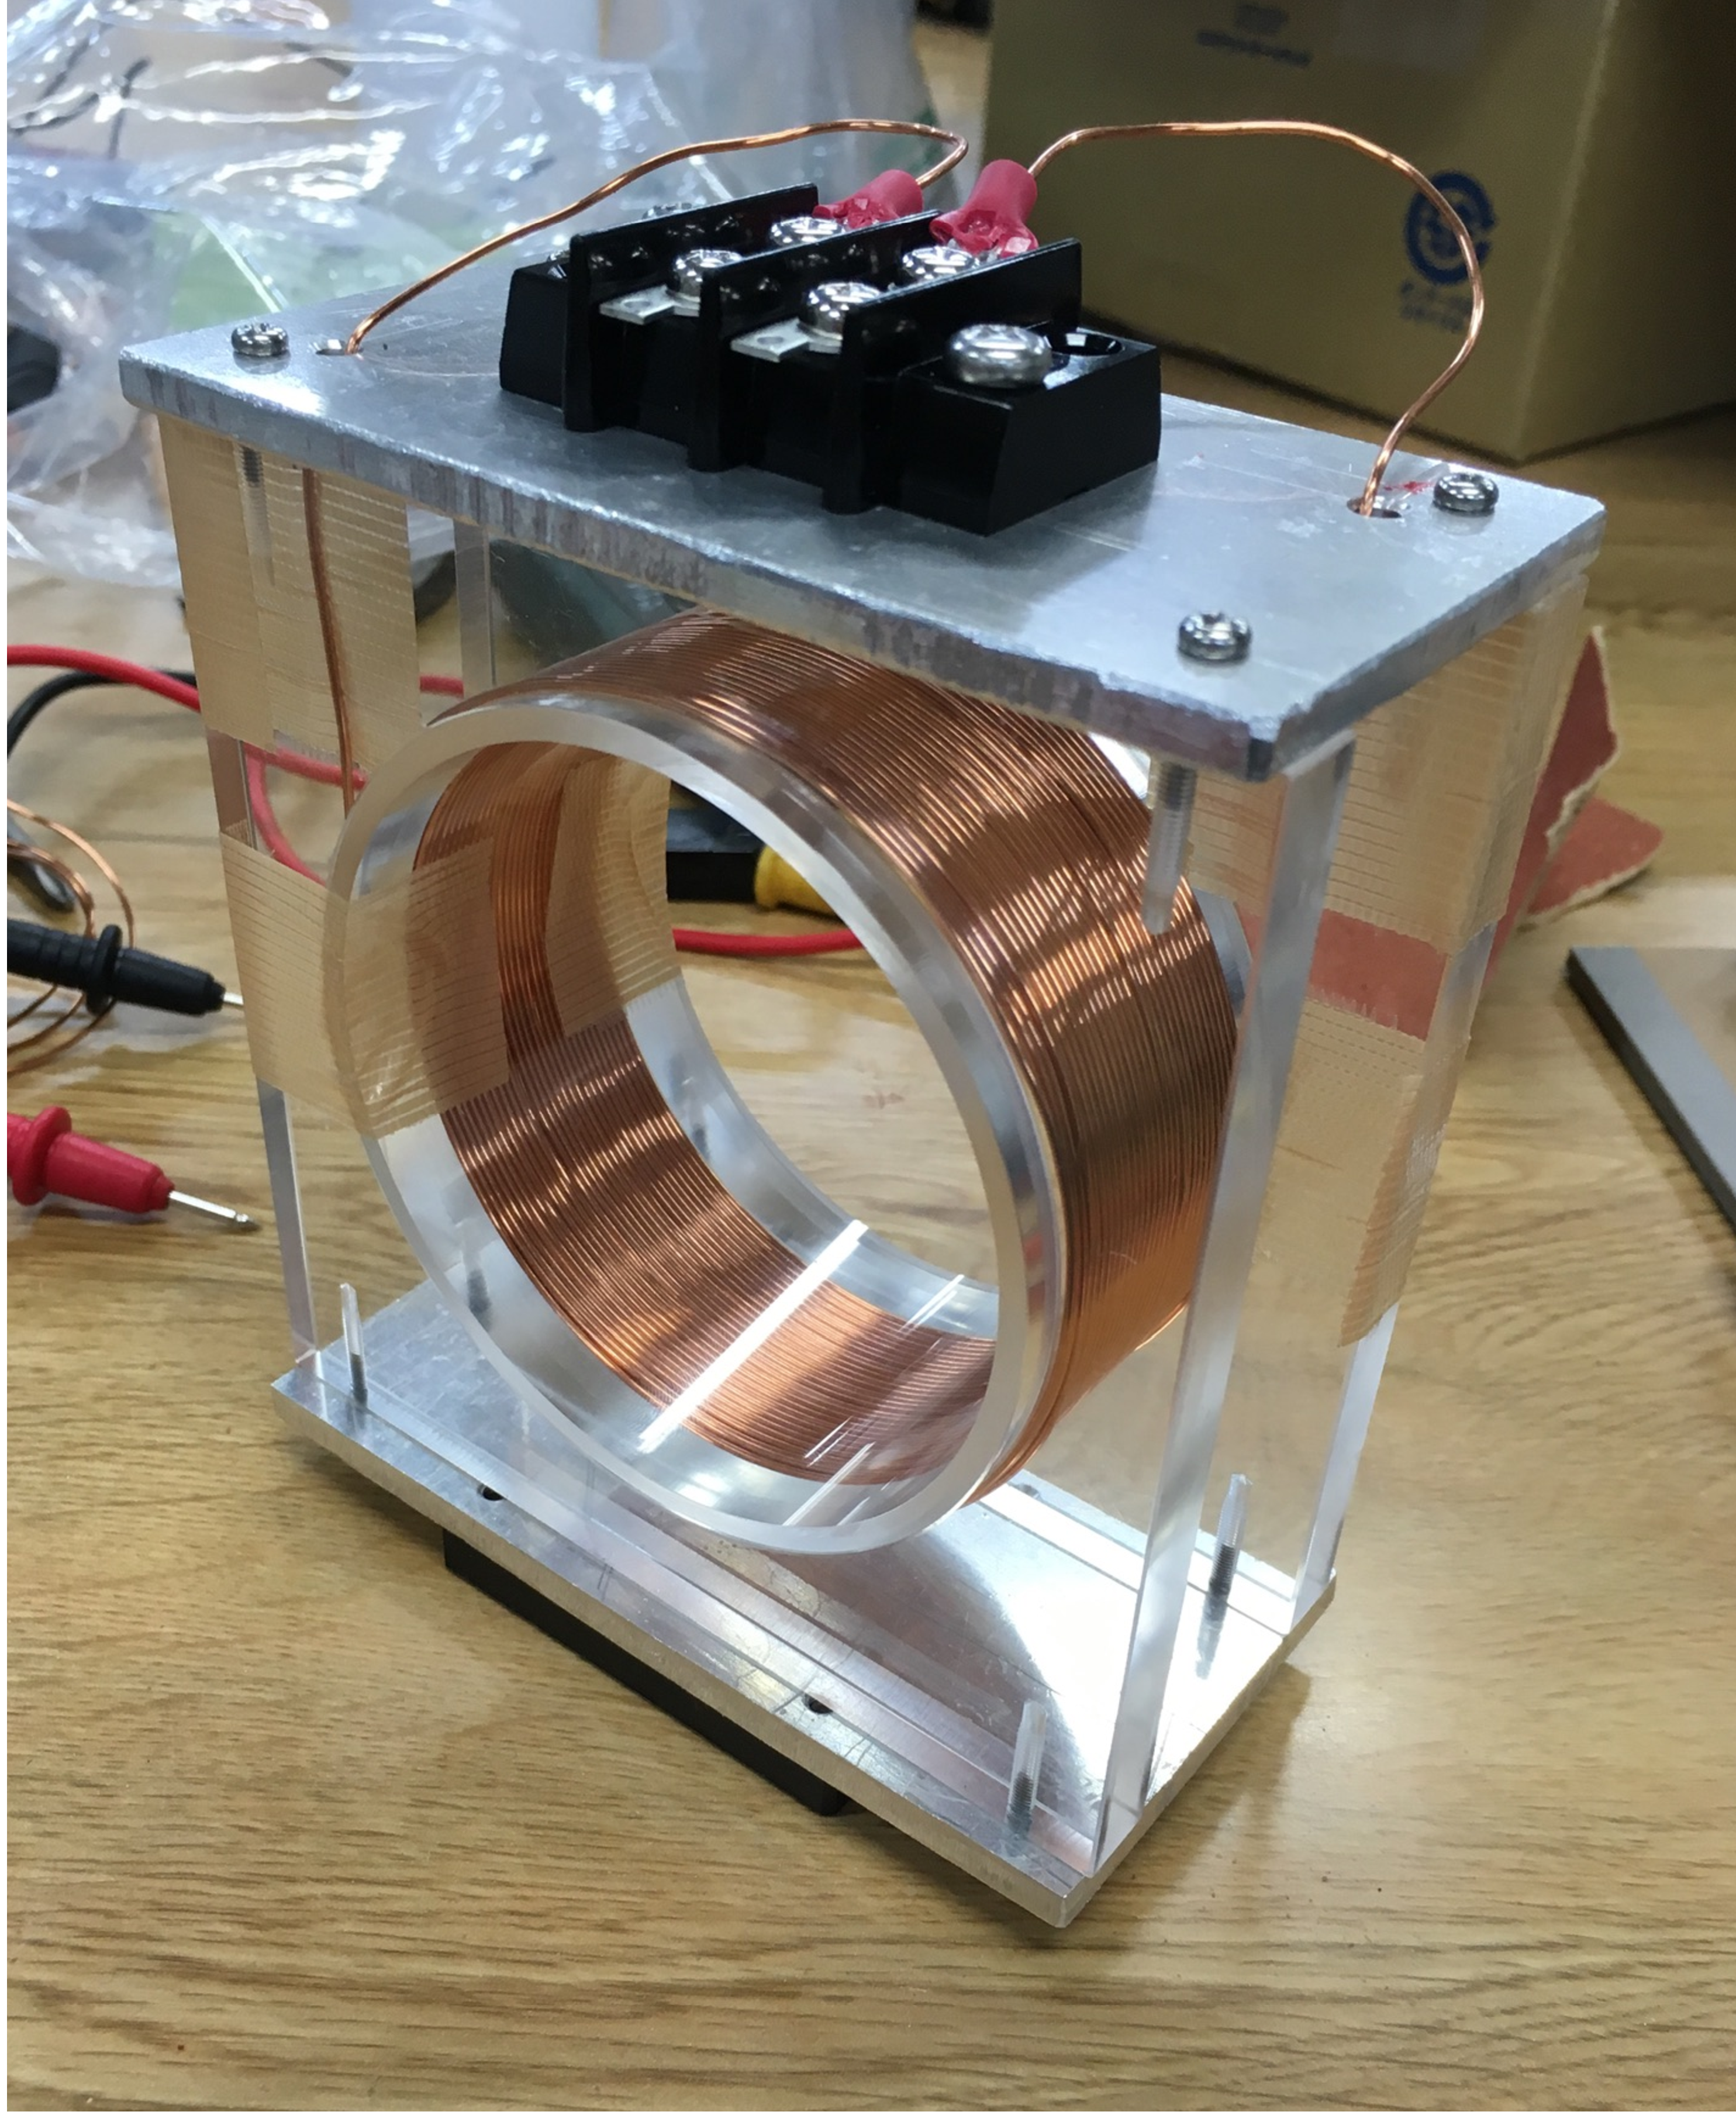
\includegraphics[width=5cm,height=6cm]{device/spinflipperphoto.pdf}\caption{自作したスピンフリッパ―}
\end{figure}



\section{位相シフタコイル}
位相シフタコイルの役割は垂直方向に磁場を作り出し、上向きスピンの中性子と下向きスピンの中性子それぞれに位相差を付けることである。
フリッパ―と同様にソレノイドコイルに定電流を流すことによって定磁場を作り出している。
\begin{figure}[H]
\centering
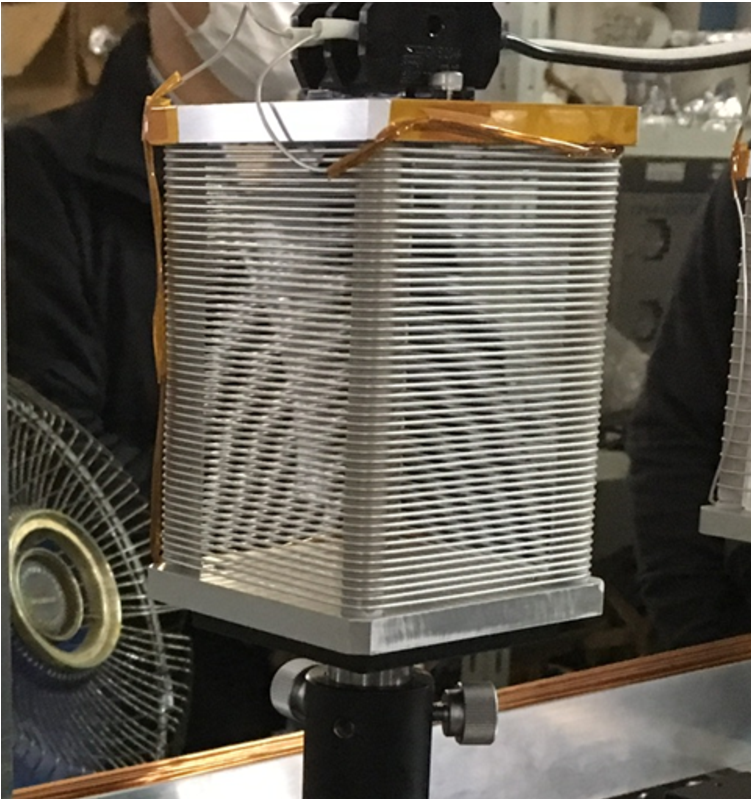
\includegraphics[width=5cm,height=6cm]{device/shifterphoto.pdf}\caption{位相シフタコイル}
\end{figure}
